\documentclass{article}
\usepackage[utf8]{inputenc}
\usepackage{graphicx}
\usepackage{float} 
\usepackage{array}
\textheight 24cm
\textwidth 16cm
\oddsidemargin 0cm
\evensidemargin 0cm
\topmargin 0cm
\hoffset -0mm
\voffset -20mm
\usepackage[]{listings}
\usepackage{amsmath}
\title{Geometric Modeling}
\author{Manuel Camargo & Mohamed Traoré &  Nicolas Gindrier}
\date{}
\begin{document}

\maketitle
\section*{Summary and presentation}
\begin{figure}[H]
   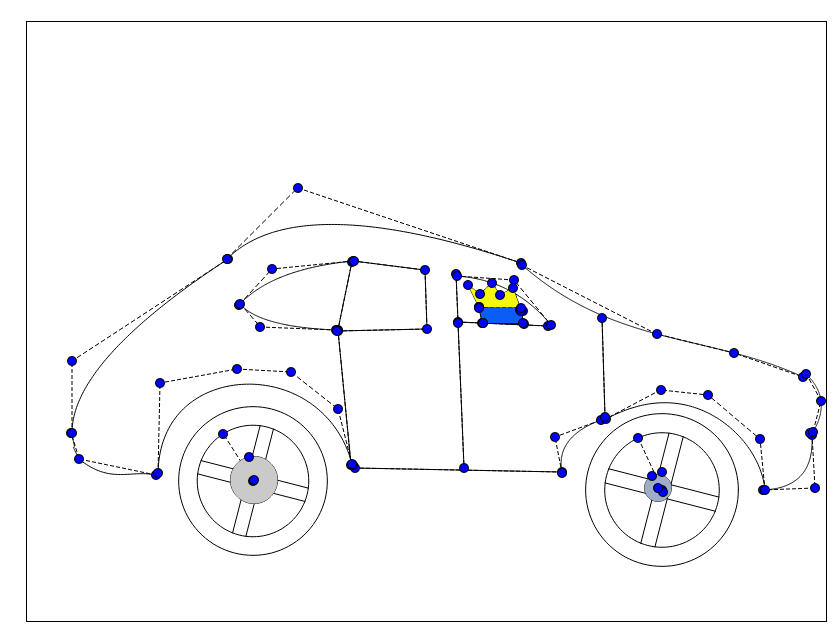
\includegraphics[scale = 0.5]{Pictures/narutovoiture.png}
\end{figure}
\section*{Organization}
We used Github. Manuel worked on parameterizations of 2D curves (Aiken Centripetal/Chordal), 1D curves and delCurve. Mohamed made 1D curves (sinus) and 2D curves (Lagrange/smooth) and Nicolas did essentially 2D curves (Hermite1-closed, Bezier and Gear, Wheel, even if there are not curves). 
\section*{Curves}
\subsection*{Curves 1-D}
\subsection*{Curves 2-D}
\subsubsection*{Bezier-Aitken}
These both curves are coded from the same way. A recursive function on the contrrol points is called. We store points in a static tab and we linked these points after. It is also used for \textit{Hermite1} and \textit{Hermiteclosed}. For \textit{Aitken} we use a uniform parameterization. 
\begin{figure}[H]
   \includegraphics[scale = 0.5]{Pictures/bezier-aitken.png}
\end{figure}
\subsubsection*{Hermite1-Hermite closed}
These curves are made with some Hermite cubic splines, based on P1, P2 and their tangent. That allows to have $C^1$ closed curves. The difficulty is to impose good direction, weight and sense for tangents.\\ 
The general formula is :
\begin{equation}
  \left\{
  \begin{aligned}
    D_{xi} = l L_1 + m L_2\\
    D_{yi} = l L_1 \dfrac{Y_{i+1} - Y_{i}}{X_{i+1} - X_{i}} + m L_2 \dfrac{Y_{i} - Y_{i-1}}{X_{i} - X_{i-1}}\\
  \end{aligned}
  \right.
\end{equation}
We adapt it for the first and the last point. Moreover $\dfrac{Y_{i+1} - Y_{i}}{X_{i+1} - X_{i}}$ is bounded.\\
l and m are equal to 1 or -1 according to tests of the form $X_{i+1} - X_{i}$, that changes the sense of the curve.\\
$L_1$ and $L_2$ are the weight of derivatives, they are a projection. Actually this is a weighted average. \\%from nico to nico : scheme

\begin{figure}[H]
   \includegraphics[scale = 0.5]{Pictures/hermite.png}
\end{figure}
\subsubsection*{Wheel-Gear}
It is not really curves. The goal here is to play with the variable \textit{frame}. We are midway between cartoon and CAD.\\
In both cases \textit{frame} is traduced as rotation speed. \\
For \textit{Wheel} we draw two circles. We use the points of the little circle in scrolling the array according to \textit{frame}. To draw a radius we link a point of the array at the size(array)/2 point. In playing with that and modulo we can draw a rolling wheel.
For gear we implicitely use a rotation matrix. We have three angles (see scheme) : alpha, to draw the gear, beta, to make rolling the gear, depending on frame and an angle depending on the mouse position (it is for follow the mouse and engage another gear). These three angles are added. \\
Actually there is a repetition of 4 points, at every rotation we choose to add or substract at the radius the half-size of a teeth. Besides, the radius is computed to have an whole number of teeth.\\% scheme of angles
So the user can drow a gear in clicking one or two times to chose the sense of rotation (an odd number for clockwise, otherwise counter-clockwise) then right-click for the radius (in fact almost the radius as above explained).
\begin{figure}[H]
   \includegraphics[scale = 0.5]{Pictures/gear-wheel.png}
\end{figure}

\subsection*{others} %for example DelCurve
\section*{Prospects}
We had a lot of ideas but some of them have not been made. It was because of time, or because we fear to modify some files. We do not master the architecture of the whole project. For example matstering scene.h would allowed many things, like to save. 
\end{document}
